%%%%%%%%%%%%%%%%%%%%%%%%%%%%%%%%%%%%%%%%%%%%%%%%%%%%%%%%%%%%%%%%%%%%%%
% LaTeX Example: Project Report
%
% Source: http://www.howtotex.com
%
% Feel free to distribute this example, but please keep the referral
% to howtotex.com
% Date: March 2011 
% 
%%%%%%%%%%%%%%%%%%%%%%%%%%%%%%%%%%%%%%%%%%%%%%%%%%%%%%%%%%%%%%%%%%%%%%
% How to use writeLaTeX: 
%
% You edit the source code here on the left, and the preview on the
% right shows you the result within a few seconds.
%
% Bookmark this page and share the URL with your co-authors. They can
% edit at the same time!
%
% You can upload figures, bibliographies, custom classes and
% styles using the files menu.
%
% If you're new to LaTeX, the wikibook is a great place to start:
% http://en.wikibooks.org/wiki/LaTeX
%
%%%%%%%%%%%%%%%%%%%%%%%%%%%%%%%%%%%%%%%%%%%%%%%%%%%%%%%%%%%%%%%%%%%%%%
% Edit the title below to update the display in My Documents
%\title{Project Report}
%
%%% Preamble
\documentclass[paper=a4, fontsize=11pt]{scrartcl}
\usepackage[T1]{fontenc}
\usepackage[utf8]{inputenc}
\usepackage{amsmath,amsfonts,amsthm} % Math packages
\usepackage[pdftex]{graphicx}	
\usepackage{url}
\usepackage[skip=2pt]{caption} % example skip set to 2pt
\usepackage[croatian]{babel}
\usepackage{listings}
\usepackage{enumitem}

%%% Custom sectioning
\usepackage{sectsty}
\allsectionsfont{\centering \normalfont\scshape}


%%% Custom headers/footers (fancyhdr package)
\usepackage{fancyhdr}
\pagestyle{fancyplain}
\fancyhead{}											% No page header
\fancyfoot[L]{}											% Empty 
\fancyfoot[C]{}											% Empty
\fancyfoot[R]{\thepage}									% Pagenumbering
\renewcommand{\headrulewidth}{0pt}			% Remove header underlines
\renewcommand{\footrulewidth}{0pt}				% Remove footer underlines
\setlength{\headheight}{13.6pt}


%%% Equation and float numbering
\numberwithin{equation}{section}		% Equationnumbering: section.eq#
\numberwithin{figure}{section}			% Figurenumbering: section.fig#
\numberwithin{table}{section}				% Tablenumbering: section.tab#

%%% Maketitle metadata
\newcommand{\horrule}[1]{\rule{\linewidth}{#1}} 	% Horizontal rule

\title{
		%\vspace{-1in} 	
		\usefont{OT1}{bch}{b}{n}
		\normalfont \normalsize \textsc{Fakultet Elektrotehnike i Računarstva} \\ [25pt]
		\horrule{0.5pt} \\[0.4cm]
		\huge 4. Domaća zadaća - ROVKP \\
		\horrule{2pt} \\[0.5cm]
}
\author{
		\normalfont 								\normalsize
        Vinko Kolobara\\[-3pt]		\normalsize
        \today
}
\date{}


%%% Begin document
\begin{document}
\maketitle

\section{Zadatak: Rad s kolekcijskim tokovima}
Koliko je bilo ulaznih datoteka senesorscope-monitor-xx.txt?\\
97\\

- Koliko se zapisa nalazi u izlaznoj datoteci?\\
4726643\\

- Kolika je veličina izlazne datoteke?\\
407.800.597 byte-a\\


\pagebreak

\section{Zadatak: Obrada podataka programskim okvirom Apache Spark}
1. Koje je najnepopularnije žensko ime kroz čitav period i države?\\
Anaissa\\

2. Kojih 10 muških imena su najpopularnija kroz čitav period i države?\\
James, John, Robert, Michael, William, David, Richard, Joseph, Charles, Thomas\\

3. U kojoj državi je 1946. godine rođeno najviše djece oba spola?\\
NY\\

4. Kakvo je kretanje broja novorođene ženske djece kroz godine? Rezultat je (sortirana) lista tipa Pair2 (ključ
je godina, a vrijednost je broj novorođenčadi)\\

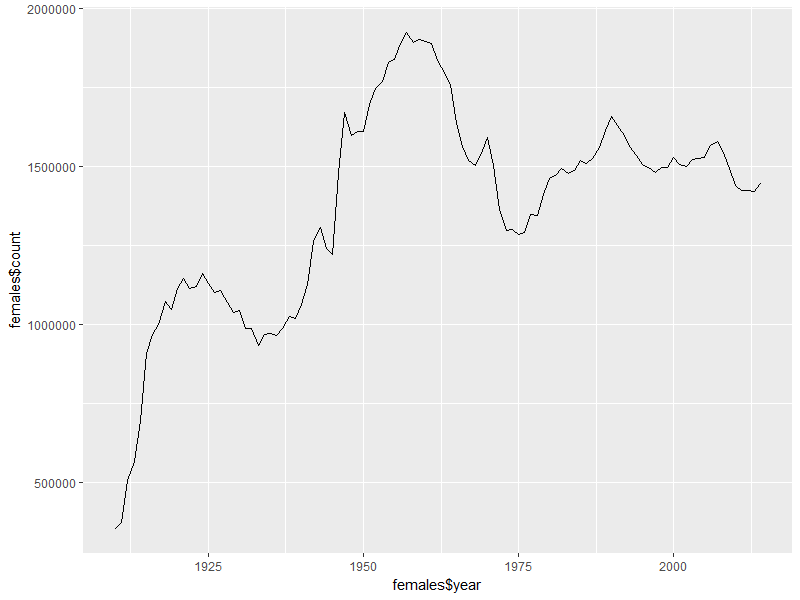
\includegraphics[width=\textwidth]{females.png}

5. Kakvo je kretanje postotka imena Mary kroz godine? Rezultat je (sortiran) skup tipa Pair2 (ključ je godina,
a vrijednost je postotak). Pri tome iskoristite polje iz prethodnog pitanja.\\

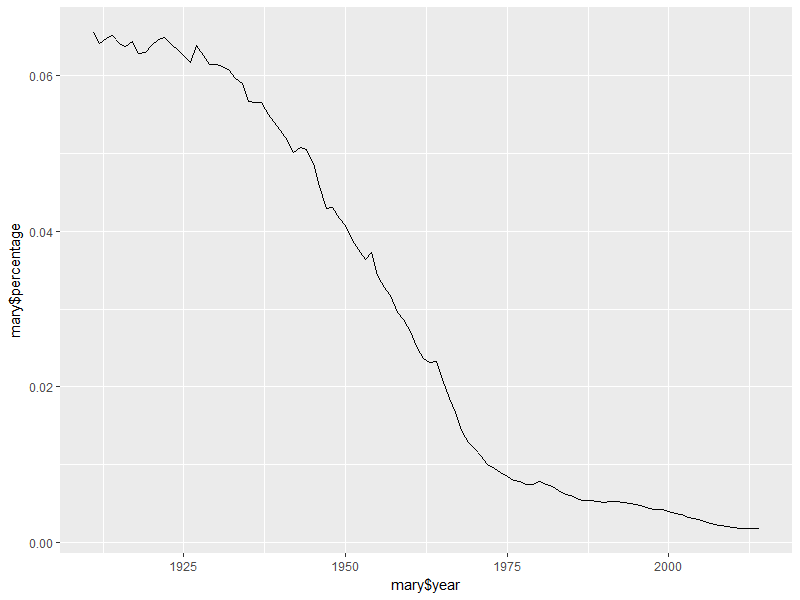
\includegraphics[width=\textwidth]{mary.png}

6. Koji je ukupni broj rođene djece u cjelokupnom periodu u svim državama?\\
298883326\\

7. Koliki je broj različitih imena koja se pojavljuju u zapisima?\\
30274

\pagebreak

\section{Zadatak: Obrada toka podataka programskim okvirom Apache Spark}

Koliko često (u sekundama) nastaje novi direktorij na disku?\\
Svakih 10 sekundi.\\

Koliko često (u sekundama) se pokreće izračun?\\
Svakih 10 sekundi.\\

Može li vrijednost parametra solarPanelCurrent neke stanice biti manja u nekom direktoriju nego u
njegovom neposrednom prethodniku. Zašto?\\
Može, svaki sljedeći direktorij za izračun uzima zadnjih 60 sekundi (svakih 10 sekundi), tako da je moguće da se maksimum prethodnog nalazio u 10 sekundi koje su prethodile trenutnom prozoru.\\

Kako se kreću vrijednosti parametra solarPanelCurrent neke postaje u prva 3 direktorija koji su nastali?
Zašto?\\
Brzo se povećava dok ne dosegne neku uobičajenu vrijednost, a razlog tome je vjerojatno što se tada tek uključio senzor i uređaj na kojem mjeri.

\end{document}